%%%%%%%%%%%%%%%%%%%%%%%%%%%%%%%%%%%%%%%%%
% University/School Laboratory Report
% LaTeX Template
% Version 3.1 (25/3/14)
%
% This template has been downloaded from:
% http://www.LaTeXTemplates.com
%
% Original author:
% Linux and Unix Users Group at Virginia Tech Wiki 
% (https://vtluug.org/wiki/Example_LaTeX_chem_lab_report)
%
% License:
% CC BY-NC-SA 3.0 (http://creativecommons.org/licenses/by-nc-sa/3.0/)
%
%%%%%%%%%%%%%%%%%%%%%%%%%%%%%%%%%%%%%%%%%

%----------------------------------------------------------------------------------------
%	PACKAGES AND DOCUMENT CONFIGURATIONS
%----------------------------------------------------------------------------------------

\documentclass{article}

\usepackage[version=3]{mhchem} % Package for chemical equation typesetting
\usepackage{siunitx} % Provides the \SI{}{} and \si{} command for typesetting SI units
\usepackage{graphicx} % Required for the inclusion of images
\usepackage{natbib} % Required to change bibliography style to APA
\usepackage{amsmath} % Required for some math elements 
\usepackage{todonotes}
\usepackage{wrapfig}
\usepackage{caption}
%\usepackage{chemmacros}
\usepackage[export]{adjustbox}
\usepackage{pbox}
\usepackage{listings}
\lstset{
captionpos=b,
language=c,
stepnumber=2,
tabsize=2,
frame=single,
label=DescriptiveLabel,
% upquote=true,
aboveskip={1.5\baselineskip},
columns=fullflexible,
showstringspaces=false,
extendedchars=true,
breaklines=true,
showtabs=false,
showspaces=false,
showstringspaces=false,
% identifierstyle=\ttfamily,
% keywordstyle=\footnotesize,
% keywordstyle=\font\ttfamily,
% keywordstyle=\color[rgb]{0,0,1},
% commentstyle=\color[rgb]{0.133,0.545,0.133},
% stringstyle=\color[rgb]{0.627,0.126,0.941},
% basicstyle=\color[rgb]{0,0,0},
basicstyle=\footnotesize,
}
\usepackage{geometry}
\newgeometry{left=2cm, right=2cm, bottom=2cm, top=3cm}
\setlength\parindent{0pt} % Removes all indentation from paragraphs

\renewcommand{\labelenumi}{\alph{enumi}.} % Make numbering in the enumerate environment by letter rather than number (e.g. section 6)

%\usepackage{times} % Uncomment to use the Times New Roman font

%----------------------------------------------------------------------------------------
%	DOCUMENT INFORMATION
%----------------------------------------------------------------------------------------

% \title{Energy Aware Software} % Title

% \author{\textbf{Principal investigator}: Simon Holmbacka\\ \AA{}bo Akademi University, Embedded Systems Laboratory} % Author name

\begin{document}
\huge{Energy Aware Software}
% \normalsize\textbf{Principal investigator}: Dr. Simon Holmbacka\\ 
% \textbf{Project starting time}: 01.09.2017\\
% \textbf{Duration of the project}: 48 months\\
% \textbf{Site of research}:\\
% \textit{\AA{}bo Akademi University} \\
% \textit{Faculty of Science and Engineering}\\
% \textit{Embedded Systems Laboratory}\\
% \textit{Vattenborgsv\"{a}gen 5 20500 Turku, Finland}\\

\begin{table}[h]
\begin{tabular}{  l  l  }
\pbox{15cm}{\normalsize\textbf{Principal investigator}: Dr. Simon Holmbacka\\\textbf{Project starting time}: 01.09.2017\\\textbf{Duration of the project}: 48 months\\} & 
\pbox{10cm}{\textbf{Site of research}:\\\textit{\AA{}bo Akademi University, Turku, Finland}\\\textit{Faculty of Science and Engineering}\\\textit{Embedded Systems Laboratory}}
 
\end{tabular}
\label{tab:strconf}
\end{table}
\normalsize
\textbf{Sites for research cooperation:}
\begin{table}[h]
\begin{center}
\begin{tabular}{  l  l  }
\pbox{10cm}{\textit {IETR - INSA Rennes }
\includegraphics[width=0.4cm]{fig/fra.png} \\\textit {Institut d'Electroniques et de T\'{e}l\'{e}communications}\\\textit{Rennes,  France}} & 
\pbox{10cm}{\textit {TU Wien }
\includegraphics[width=0.4cm]{fig/aus.png} \\ \textit{Institute for Software Technology and Interactive Systems}\\\textit{Vienna, Austria}}   \\ \\
\pbox{10cm}{\textit{FernUniversit\"{a}t in Hagen }
\includegraphics[width=0.4cm]{fig/ger.png} \\ \textit{Fakult\"{a}t f\"{u}r Mathematik und Informatik}\\ \textit{Hagen, Germany}} & 
\pbox{10cm}{\textit{Uppsala University }
\includegraphics[width=0.4cm]{fig/swe.png} \\\textit{Department of Information Technology}\\\textit{Uppsala, Sweden}} \\ 
\end{tabular}
\label{tab:strconf}
\end{center}
\end{table}

\date{\today} % Date for the report

% \maketitle % Insert the title, author and date
\normalsize
\section{Executive Summary}
Energy consumption is currently a challenge in all domains of computer systems.
IoT, cyber physical systems and other mobile systems demand solutions to lower the energy consumption while keeping the same amount of computations,
and high end systems, servers and exa-scale computing demand more computations for the same energy.
These problems were traditionally solved by the hardware evolution, but since we now witness the end of the Dennard scaling \cite{Dennard:74} it is no longer a viable option.
As the improvement in semi-conductors no longer keep the required phase, evolution in energy efficiency must be shifted to the software.
Our vision in this research is to improve energy efficiency of computer systems by involving the application software in the resource allocation decision -- this branch of self-awareness is called making the software energy aware.
Energy aware software form a stronger link between applications and the runtime system in form of an information flow used to steer the resource allocation.
This increases the self awareness of software and is required for the research community to take the next step into energy efficient computing.

\section{Rationale}
From tiny embedded systems to large scale server farms and diverse IoT systems, energy efficiency is becoming the main struggle for system usability, expansion, reliability and scalability.
The drivers for solving the issues differ depending on the area of focus;
%\todo[inline,color=green]{Here comes the current problems with high energy consumption:}
%embedded
the very usability of battery powered devices depends on its ability to provide the user with the satisfactory experience while consuming the minimal amount of energy.
%Desktop
Desktop and laptop systems require high levels of energy efficiency to lower noise levels from active cooling, increase the reliability by reducing the heat and minimize the electric bill.
%server
On the larger scale, the rapid expansion of large scale servers is not in line with ecological development, and now contributes to over 2\% of the total energy consumption in the US\footnote{Statistics according to the U.S. Office of Energy Efficiency \& Renewable Energy: http://energy.gov/eere/femp/resources-data-center-energy-efficiency}, with Facebook alone releasing 650k tonnes of carbon annually\footnote{https://sustainability.fb.com/en/our-footprint/}.
%exascale
Lastly, without increased energy efficiency, high performance computing centers cannot reach exa-scale performance.
The US Department of Energy\footnote{http://ascr-discovery.science.doe.gov/2014/11/exascale-road-bumps/} have defined a maximum power envelope of 20 MW for a single data center, but with current technology, an exa-scale computing center would require over 7000 MW.\smallskip

%\todo[inline,color=green]{Here comes that HW was the solution yesterday but not anymore:}
To provide continuous performance increase in computing systems, the clock frequency wall was avoid in the beginning of the 2000s by the introduction of multi-core based systems. 
This led to a new challenge in mid-2000s: the CPU power wall \cite{Danowitz:12,Wang:13}. 
Indeed, due to physical limitations of semiconductor materials, the power dissipation of a fixed chip area is limited. 
With the evolution of semiconductor device fabrication, from a 10$\mu$m manufacturing process in the 70s until the commercialization of 14nm based technology in 2015, more transistors are squeezed into a smaller silicon area which increases power density \cite{5514312}. 
This eventually leads to dark silicon, when all the components of a chip can not be operated at the same time due to its power dissipation and generated heat. 
The effects of the power wall was until now limited by the design of more energy efficient transistors with for example lower voltage levels.
This had the advantage to increase the transistor efficiency in proportion to the increase of transistor density, a phenomenon called the Dennard scaling \cite{Dennard:74}. 
However the current increase of the transistor efficiency is not any more proportional to the increase of transistor density \cite{Wang:13}, 
and the semiconductor device fabrication is currently in a post-Dennard scaling area, where a substantial increase of the performance of computing
systems can not be obtained before solving the current power dissipation and related energy consumption issues.\smallskip
%Hardware has historically been the solution to these problems, but the energy evolution in hardware is not anymore proportional to the performance due the end the Dennard scaling  \cite{Dennard:74}.
%This means that as transistors become smaller, energy efficiency is not any more improved by transistor technology alone, such that the power remains in proportion to the chip density. 
%A typical processor chip has a limited power envelope of roughly 250W before the heat dissipation damages the silicon.
%which means that all chip area cannot be utilized simultaneously, a phenomenon called ``dark silicon''.
%Traditionally, chip manufacturers have continuously lowered the chip voltage to solve the energy density problem,
%but physical limitations to reach millivolt switch voltage in transistors prohibits chip manufacturers from operating on lower voltages than about 1V. 
%Furthermore on the other front, hardware development, alone, in form of battery development in mobile phones also lacks the ability to keep up with the progress in processor capacity \cite{CPUCapacity,BatteryCapacity}.
%This means that the increased performance capabilities of the mobile processor is evolving far quicker than the battery capacity.
% Thus, hardware evolution in terms of energy efficiency cannot keep up with the phase of the increased performance demand.\smallskip

%\todo[inline,color=green]{Here comes what is needed to solve the problem:}
In order to solve the mentioned problems in this interdisciplinary domain, software must inevitably be involved to make computer systems energy efficient again!
The key challenge is to utilize the available hardware resources as efficiently as possible.
Since general purpose applications have a very dynamic behavior, a runtime environment must continuously adjust the usage of the resources based on the execution of the applications.
In Linux based systems, attempts have been made to incorporate this behavior by using clock frequency scaling and deep sleep states to scale the hardware resources according to the demand. 
The problem with the existing approaches is that the resources are allocated based on poor metrics.
There is no interoperability between applications and the runtime system, and resources are usually allocated based on indirect metrics such as the system \textit{workload}.
Such a metric does not describe performance demands in applications, and therefore often causes incorrect resource allocation and thus energy waste \cite{HolmbackaDasip, HolmbackaHipeac}.
\smallskip

\begin{wrapfigure}{br}{8.5cm}
%   \begin{center}
%     \vspace{-0.8cm}
    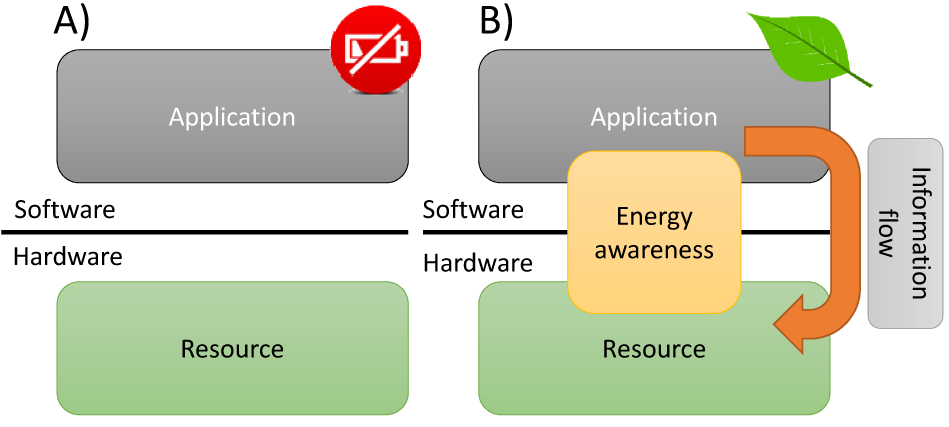
\includegraphics[width=8.0cm]{fig/EAS_Overview.png}
%   \end{center}
  \caption{A: No connection between the application and the resources B: Resource allocation based on self-awareness}
  \label{fig:EAS}
%   \vspace{-2cm}
\end{wrapfigure}

%\todo[inline,color=green]{Here comes what we do in this research:}
In this research we will extend the application software with the notion of \textit{energy awareness}.
This is a property needed to directly involve applications in the resource allocation.
Energy aware software is able to continuously report the performance demand in its own specific metric to the runtime system.
With this information, the runtime system can allocate resources (usually with clock frequency scaling and with sleep states) with a much greater accuracy than using indirect metrics such as the workload.
Energy savings as much as 50-60\% was obtained by using energy awareness in software in our previous research \cite{Holmbacka:15} on real-world Linux platforms without loosing any performance.
We are therefore confident that adding energy awareness in general purpose software can reduce the energy consumption significantly.
Figure~\ref{fig:EAS} illustrates the efforts of the research: part A) shows the current approach without any interoperability between applications and the resources.
Using this approach, resources are allocated based on the level of workload or other indirect means of metric.
Part B) Figure \ref{fig:EAS} illustrates the addition of energy awareness. 
This is the added interface between the application and the runtime system through which the application communicates.
It results in better accuracy of resource allocation, increase self awareness and lower energy consumption.\smallskip

The research area in energy efficient computing is a broad domain spanning several levels of hardware from IoT to Exascale.
The commonality is, however, the ability to propagate information from the highest software layer to the runtime system, and to the hardware.
Throughout all computing domains in the area of energy efficient computing, we have identified three critical challenges to address in our research further specified in sections \ref{sec:self}, \ref{sec:inter} and \ref{sec:smart}.

\subsection{Self awareness}
\label{sec:self}
Applications must be able to properly express their intentions in terms of performance requirements during an execution. 
The requirements are added to the application software in form of performance meta-data -- a performance goal the application is due to achieve. 
The challenge is therefore to provide a framework with the capability of handling and expressing performance meta-data in an interdisciplinary domain.
As previously mentioned, the traditional way of solely monitoring the workload is a very inaccurate and often counter-productive both in terms of performance and energy.
We tackle this challenge by allowing the applications to express the resource requirements internally.
This means that the application should include a small part of code -- the meta-data -- which expresses the intention of the application in its own understanding of performance.
For example, the end user of a video decoder is satisfied in case the decoder produces a framerate of 25 fps because of properties in the human eye and the understanding of moving pictures. 
A higher framerate is therefore energy waste while not producing any higher satisfaction for the end user.
Therefore, we will investigate the types on meta-data needed to describe the intentions of an application sufficiently accurate.
One of the challenges is to obtain a sufficiently descriptive form of meta-data that can be generalized to any new- or legacy application.
Once the meta-data descriptions have been established, the injection of the data into both new- and legacy applications must be achieved fairly effortless in order for the programmers to make the additional effort.
A trade-off between descriptiveness and programmer effort is to be expected.

\subsection{Interoperability for energy efficiency}
\label{sec:inter}
The interoperability challenge in the domain of energy awareness in application software is to create an ecosystem capable of exchanging information about the intentions of an application to the runtime software layer. Secondly, the exchanged information must be interpreted by the runtime layer to make sensible decisions regarding the resource allocation.
Since applications in general are dynamic, the performance of the application depends on a wide set of factors such as memory intensity, use of caches, user interrupts, the data sizes and data types used, interaction with other applications etc. 
This means that the performance of an application cannot be guaranteed with fixed resources.
In order to adapt the resources allocated to the application, the performance of the application must be monitored at runtime.
In case the currently allocated performance is either too high or too low, the monitor reports this issue to the controller which allocates or deallocates resources to accommodate for the real resource requirement.
We recognize therefore the need for a proper monitoring framework to insure the interoperability between applications and the runtime system.
Such a framework must be detailed enough and provide sufficient tools for measuring performance, but simple enough to reduce programmer effort for using it.
Since the monitoring framework is a runtime system, significantly low overhead must be guaranteed to not interfere with the energy consumption and performance of the host system.

\subsection{Smart adaptivity}
\label{sec:smart}
Given a proper dataflow from applications to the runtime system, the final challenge is the allocation of resources. 
Allocating resources efficiently means having a knowledge of how resources of one form affects the performance of the application requesting the resources.
Even though feedback control loops is a mature area of research, the methods must be adapted and applied to the general purpose computing domain. Together with machine learning, big data and pattern recognition, smart adaptivity in the control loop helps to bring the framework of energy aware software to a broader domain of computing systems from IoT to exa-scale systems.

\subsection{Previous work}
The embedded systems lab in the \AA{}bo Akademi University has for the last six years focused on low power and energy aware software. 
During these years a special interest had been put in mobile phone processors and their significance for energy awareness in general. 
This is because it has been noted that the trend of performance requirements by far exceeds the battery capacity of a mobile device, especially since the mobile multi-core revolution \cite{BatteryCapacity,CPUCapacity}. 
This means that the performance of the hardware and the demand for performance of the user is greater than the energy a battery with limited dimensions can physically store. 
Because of the slow capacity increase in batteries, the available energy must be used more efficiently in order for such a mobile device to retain its usability.
In the thesis of the PI ``\textit{Energy Aware Software for Many-Core Systems}'' two guidelines were presented for creating energy aware software on modern many-core hardware. 
Implementing the recommendations in software has proven to reduce the energy consumption up to 50\% without degrading the performance \cite{HolmbackaHipeac}, especially on mobile multi-core hardware. 
The recommendations called ``Energy aware mapping'' and ``Energy aware resource allocation'' are used to tailor the resource allocation to the software executing, 
and a prototype runtime system was implemented as a phase of the PhD thesis. 
Using this software, practical state-of-the-art demonstrators were created, for example a low power video transcoding cloud system\footnote{Picture of the ESLab demonstrator available at https://dl.dropboxusercontent.com/u/5260559/ClusterDemo.jpg} demonstrated in the Millennium Pavilion SHOK Summit in Helsinki, and in the DIGILE Workshop ``Rolling up the Sleeves''.
Also, the Android app ``Low Energy Player'' was implemented as a state-of-the-art demonstrator and is available on Google store\footnote{https://play.google.com/store/apps/details?id=org.videolan.vlc.LEL.lite.green}
This research is intended to go beyond the state-of-the-art by the development of a programming framework for energy aware software and practical demonstrators.

\subsection{Related work}
``Low energy programming'' or ``Low power programming'' has previously existed in the form focusing on the programming paradigm or on the programming syntax. 
Guidelines from Intel \cite{IntelLowPower} suggests the use of a certain level of loop unrolling, vectorization, memory intensity cache usage etc.
for achieving maximum energy efficiency in combination with Intel compiler tools. 
Such recommendations are applied only on the algorithms in the program, and do not cover, the intention of the program for functioning efficiently together with the runtime system allocating the resources. 
The low power programming guidelines from Intel also require the programming to construct the program in a certain way in order to become energy efficient, 
and the underlying hardware architecture must be known. 
In the thesis ``Developing Energy-Aware Software'' by Brinke \cite{Brinke:15} the author describes programming languages for modularity and modeling resource consumption for software.
The \textit{awareness} of energy, is tightly bound to the application code and the programmer is expected to follow certain programming patterns to make the software energy aware.
On the contrary, the planned framework for energy efficient software requires only the insertion of meta-data in the software.
This means minimal effort of the programmer and the application algorithms can be implemented without interference from the energy awareness framework.
The resource requirements are specified using a simple library, where after the runtime environment allocates the required resources.\smallskip

The \textbf{Carbon Research Group}\footnote{http://groups.csail.mit.edu/carbon/} at MIT has developed a heartbeat framework to evaluate performance as a generic parameter in software construction.
The framework is capable of measuring performance of any application as a generic parameter by user inserted API calls to the heartbeat library. 
Measuring performance is the necessary first step when constructing a feedback-based control system. 
For example it enables the possibility to measure the framerate in a video decoder, but a controller is then needed to allocate the resources in order to keep the performance on a given setpoint. 
We consider using the heartbeat framework for measuring generic performance in our energy awareness framework, 
but we plan to extend the framework considerably in order to add the controller for allocating resources.\smallskip

The \textbf{Hardkernel} project\footnote{http://www.hardkernel.com/main/main.php} creating the Odroid family boards recently released the Global Task Scheduling (GTS) support for the ARM big.LITTLE devices. ``High performance threads'' are scheduled to the big high performance cores and ``Low performance threads'' are scheduled to LITTLE energy efficient cores based on the workload activity of the threads in order to save energy. 
Even though the activity level of a thread is an early attempt introduce energy awareness in the system, the practical results are poor. 
In other words, the scheduler most often schedule a thread on \textit{the wrong core}. 
This results not only in poor energy efficiency, but also in poor performance of the applications and poor user experience. 
We intend to use this platform as one of the reference models for our energy awareness framework because its SoC is very popular and is being used in millions of Android devices worldwide.\smallskip

Our research group is currently a partner in the \textbf{INTERSYS} project\footnote{http://iot4health.utu.fi/?p=374} dedicated to standardize and optimize interconnected IoT devices handling streaming data. Since the number of IoT devices are expected to rapidly increase in the near future, the project is extending interoperability notions for handling the massive amount of data streams from small devices to gateways and servers. 
Still missing in the field of IoT is the notion of energy awareness, which is a crucial point as most devices operate on battery-only power and are expected to operate for long time intervals. 
We intend to work closely with this project and we plan to introduce the notion of energy awareness in IoT systems.\smallskip

\textbf{EMBECOSM}\footnote{http://www.embecosm.com/} focus on providing the GCC compiler with the notion of energy efficiency, in practice this means learning which compiler flags that minimizes the energy consumption for a selected architecture. 
The outcome of this project is similar to OpenTuner \footnote{http://opentuner.org/} from MIT, which is capable of offline optimization of multi-criteria problems. 
Both projects provide a metric for offline optimization but runtime support, which we suggest, is not stated in their scope. 
Runtime optimization is critical in virtually any environment containing multi-node and heterogeneous multi-node platforms. 
This is because the data used in especially streaming applications like multi-media software is arbitrary or very difficult to predict. 
Compile time optimizations can for example not predict what kind of video format is being used in a video decoder.\smallskip

The \textbf{StarPU}\footnote{http://starpu.gforge.inria.fr/} project at INRIA Bordeaux has presented a runtime system to minimize the performance for heterogeneous architectures. 
The system builds a performance model of the implemented CUDA or OpenCL kernels based on benchmarking on CPUs and GPUs, after which the system is able to schedule the kernels onto the most performance efficient device. 
The \textbf{PEPPHER}\footnote{http://www.peppher.eu/} project has used StarPU as a backend and the outcome of the project is a tool capable of generating multi-variant tasks for StarPU (OpenMP, OpenCL etc.). 
However, StarPU only consider the optimizations in form of performance. 
When adding more complex criteria with multiple variables such as energy efficiency or monetary cost, StarPU lacks the insight to such resource allocation.

\section{Objectives and expected results}
\subsection{Objectives}
Our objectives is to address the energy consumption problem in computer systems.
In most recent systems, power managers have been implemented to scale the performance of the system according to the current resource demand.
Various implementations exist depending on the whether the system is a large cloud farm or a small IoT system, 
but main problem in current solutions is the inability to accurately express resource demands.
In mainstream Linux systems, the resource demand is measured as the utilization caused by the workload of the CPU. 
Workload in operating systems is measured as a sliding window average over an active and idle CPU as illustrated in Figure~\ref{fig:workload}. 
A high workload indicates that the system needs more resources, and the clock frequency is scaled up to decrease the workload of the CPU.
Setting the frequency can be based on different policies implemented in \textit{frequency governors}, and the most common policy is called ``ondemand''\cite{ondemand}.
This frequency governor scales the clock frequency to the maximum value as soon as a workload threshold is reached.
After this it step-wise decreases the clock frequency to the lowest frequency not exceeding the threshold.\smallskip 
\begin{wrapfigure}{br}{8cm}
  \begin{center}
    \vspace{-0.8cm}
    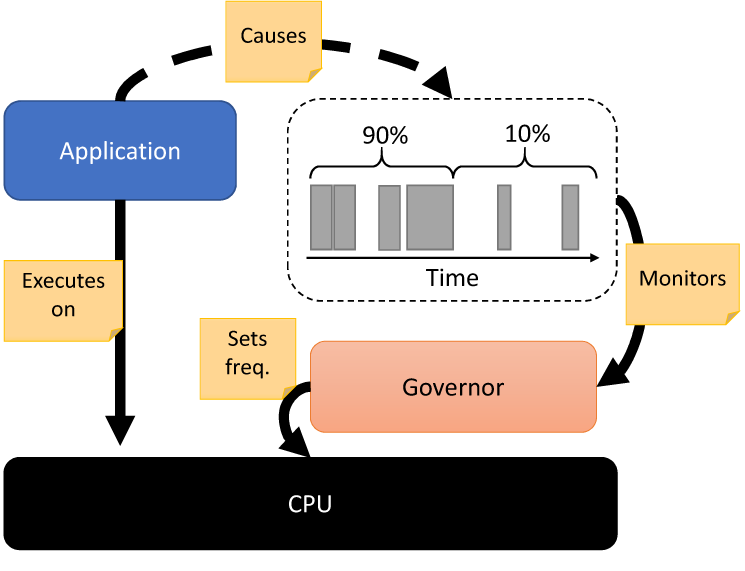
\includegraphics[width=7.5cm]{fig/WorkloadMonitor.png}
  \end{center}
  \caption{Current power management systems: The application causes a workload (illustrated by the gray rectangles), and the frequency governor scales the clock frequency according to the load level.}
  \label{fig:workload}
%   \vspace{-2cm}
\end{wrapfigure}
The problem with this approach is that the workload does not describe the performance of the applications accurately enough.
High workload does not necessary mean that an application requires more performance, it simply describes how much the application is using the CPU.
It is merely an indirect effect of executing an application as illustrated in Figure~\ref{fig:workload}.
Incorrect resource allocation result in either poor performance or in energy waste.
% For example, in case the CPU is set to decode a video, the workload will increase to 100\% as soon as the video frames are being decoded.  
% This means that the CPU is clocked to the maximum frequency as long as the frames are being decoded and the decoded frame rate is only limited by the speed of the CPU; 
% even if the required decoding rate is only 25 frames per second (fps), which the human eye is capable of observing.
% In other words, the application will be executed unnecessarily fast. 
As previous results from our work in \cite{HolmbackaHipeac, HolmbackaDasip} show, executing the application unnecessarily fast wastes significantly more energy than executing the application on a moderate, but still at a sufficiently fast, performance level.\smallskip

Other work on attempting to refine the functionality of the frequency governors was presented in \cite{Spiliopoulos:11}.
Their frequency governor the ``Green Governor'' scales the clock frequency not only based on the workload, but also in the memory intensity.
The assumption made was that higher memory intensity stalls the CPU enough to not benefit from high clock frequency.
The fundamental problem was still unsolved because the governor models the performance requirement of the application indirectly,
and in case the model does not fit the application, either excessive or insufficient resources are allocated to the application.\smallskip

What we propose is to make the application software itself energy aware and \textbf{the objectives of this research} is to develop a complete framework for programming energy aware software.
Using this software, applications become involved in the resource allocation which is a necessary step for reaching the next level of energy efficiency in computer systems.
A power management system compatible with energy aware software requires therefore an interface between application and runtime system, which is current non-existing.
This research is aimed to provide such an interface, and the necessary tools needed to use it.
Our current design recommendations for energy aware programming extends the application to signal resource requirements to the runtime system, which allocates the hardware resources based directly on the requirements rather than indirect metrics like the workload.
With this framework, resources can be allocated more efficiently leading to a lower energy consumption.

\subsection{Hypothesis}
The project states the following Hypotheses:

\begin{enumerate}
 \item Performance requirements in computer systems will continue to increase significantly faster than transistor technology and battery technology development, software must thus utilize the resources more efficiently. \vspace{-0.2cm}
 \item Energy aware software can utilize the hardware resources more efficiently because hardware resources are allocated based on actual performance requirements.\vspace{-0.2cm}
 \item Software can be made energy aware with minimal performance overhead and minimal programmer efforts.\vspace{-0.2cm}
 \item 50\% of energy can be saved using energy awareness in software.
\end{enumerate}



\subsubsection{Previous work on energy aware software}
In previous work, Eyerman et al. \cite{Eyerman:09} claim that no single throughput metric is fundamentally generic for multiprogram workloads. 
Performance should instead be expressed as related to the internal single case-study; a direction adopted in this research. 
We plan to integrate this direction of thinking into user defined meta-data that expresses resource requirements in software.\smallskip

In early research, a high-level language CQML \cite{Aagedal:01} was suggested for describing QoS requirements integrated in UML. 
CQML links a high level QoS description to system performance, and can describe system actions based on the result. 
Applications specify a performance setpoint and a lower bound acceptable performance level in context of the application. 
Applications then monitor own performance and signal this value to the QoS manager periodically. 
Similar notations as this the language will be considered in this research to describe QoS in applications, 
but more focus will put on the link between applications and hardware resources in a single computer system.
Our methods for energy aware programming will not be strongly tied to a certain programming language and the framework itself will have the flexibility to be integrated from various environments such as servers and PCs and Android.\smallskip

% Hoffmann et. al propose heartbeats \cite{Hoffmann:10} as a generic performance parameter. 
% The heartbeats are setup by including a set of heartbeat API calls in applications, which are used to monitor the application performance. 
% By calling the heartbeat API on suitable places in the applications such as large loops, a notion of the update interval between API calls is created. 
% The heartbeat API registers multiple applications and the outside system monitors the heartbeat of each application separately. 
% Heartbeats is a suitable candidate, and fully compatible as a performance parameter in our research framework.
% An application can register a setpoint heartbeat after which the heartbeat monitor is used to derive the actual performance in heartbeats. 
% Earlier work by Vetter et al. \cite{Vetter:02} presents a similar approach, but by including performance assertions directly into the code. 
% Based on the assertions, the application can adapt itself in case significant performance is not achieved.
% The system allowed, however, only internal monitoring of the performance, and a runtime system was not in the scope.

On the other hand, runtime systems for minimizing energy consumption in computer systems have been previously proposed.
The PowerDial \cite{Hoffmann:11} approach allows graceful degradation in applications based on current application performance measured in heartbeats \cite{Hoffmann:10}. 
The system transforms application parameters (such as peak-signal-to-noise in a video) into dynamic control variables stored in the application itself. 
A callback function is inserted into the application using which the controller is able to adjust the control variables according to performance and policies.
A heartbeat feedback monitors the execution and reports on the updated performance of the application. 
Also, the work by Segovia \cite{Segovia:11} suggests graceful degradation of the application QoS by monitoring a happiness value from the application. 
Based on this value, the runtime system can degrade quality points in the application in order to achieve the requested QoS. 
Our planned runtime system is inspired by the same approach to treat input signals from applications: the performance is transformed into a generic parameter – QoS – upon which the controller acts.
In contrast, our controller uses no graceful degradation in the applications, but the actual hardware actuators to allocate resources.\smallskip

In previous research, there have been a strong separation between monitor and control.
Several research projects offer the opportunity to monitor an executing application, but supports no control of the hardware.
On the other hand, many controller-based research project do not support any proper framework for declaring meta-data requirements and monitoring of the execution.
This research project will tie both parts together with the main focus on reducing the energy consumption with minimal programmer effort -- an effort not previously done.
Our research project will also make the proper balance between academic research and practical usability,
which means that there is both a focus on planning the long term usage of the framework in terms of capabilities and scalability, but also practical efforts to enable a programmer to pick up the tools and start developing energy aware software in the industry.\smallskip

\section{Expected scientific and societal impacts and potential breakthrough of the research}
Our expected impact on the research community is to address the energy awareness in software. 
In other words, the need for communication between the application layer and the runtime environment. 
% We expect to determine the information flow needed to create energy aware software especially for heterogeneous architectures. 
% \todo{How with the heterogeneous issue? Is it part of this plan?}
Our potential breakthrough is to introduce \textbf{energy awareness as natural part of programming}.\\ 
For decades it has been a natural step to introduce meta-data in the software for creating parallel programs. 
The programmer has been willing to add \#pragmas in OpenMP, Keywords in Cilk or Initializations in OpenCL to create parallel software because of the minimal programming effort and significant performance gain. 
We intend to extend this notion to energy awareness, and demonstrate the potential reward in terms of energy efficiency. 
Furthermore, the development of runtime systems becomes more straight forward. 
Without energy aware programming as the underlying notion, runtime systems in any domain have no common ground on which the decision making is based. 
Optimizations remain based on ad-hoc ideas and ``hacked'' hard-code which is usually not portable between either domains or even between different architectures. 
Even though the implementation of the runtime systems between domains can be different, the core idea of resource allocation decisions based on energy aware programming remains common. 
With this common denominator, runtime systems engineers between projects and domains can incorporate shared ideas for implementing new, or improving existing runtime systems. 
For example the GTS scheduler appearing in most high-end Android phones and tablets is currently highly inefficient due to a poor decision making model. 
Moreover, its implementation model is completely isolated from any other runtime system – leaving it highly unportable. 
By introducing the notion of energy aware programming, the development of runtime systems needed in any modern computer system has the potential to shift from an ad-hoc single-purpose environment to a sharing environment where engineers have a common platform to cooperate on.

\subsection{Applicability}
\begin{itemize}
 \item Energy efficient programming: Today most guidelines for energy efficient programming is driven by creating code with efficient algorithms such as using loop unrolling, SIMD vectors, compiler options etc., which generates software specifically for a given platform. 
 By instead relying on application meta-data describing software requirements, similarly as Cilk and OpenMP handle forking and joining task, resource allocation is based on what the software actually needs instead of blindly following the workload of the system.
 \item Performance portability: one of the major obstacles within the embedded industry is the high portability costs of software which is due to the requirements for high customization of software to particular embedded architectures. 
 With the suggested energy awareness framework, the mapping and scheduling decisions are shifted from the developer to the runtime system. 
 This allows a more architecture generic programming paradigm while still keeping the performance of dedicated code.
 \item Development of runtime systems: Using the energy awareness framework, the development time of runtime systems is not only decreased but also more standardized. 
 Even potential for automatic runtime system generation emerges as a result of standardizing the foundation.
 \item 
%  Fog computing is currently being proposed as an implementation framework for the IoT. 
%  In the fog heterogeneous computing nodes are scattered in the network to enable computations neared to the source to guarantee real-time properties. 
 IoT systems are one the most energy-prone fields of computer engineering because many of such systems are designed to run for long intervals without being connected to the power grid. 
%  Currently there are no standardized mechanism for declaring energy awareness in IoT systems. 
 The framework for energy aware programming is extendable to IoT system as well because the paradigm only requires the ability of inserting resources requirement meta-data into the application software. 
\end{itemize}

\subsection{Critical points for success}
Our intension is not only to provide theoretical insights into energy aware software, but also the framework needed to enable the programming.
To ensure success, the critical points and risk factors are listed as follows:
\begin{itemize}
  \item \textit{Software design is infeasible}. With an infeasible design, the intended research results cannot be achieved without a major re-design.
  With our previous experience in energy aware software, and the results gathered we are confident about the main directions in the research. Although we intend to monitor the feasibility early in the project to ensure an eventual re-design in as early stages as possible.\vspace{-0.2cm}
  \item \textit{Learning curves lead to delays}. Learning new methods and tools is always a challenge. By exceeding the time budget in methods and tools, the project can be delayed.
  Our lab environment keep up-to-date with tools and methods by weekly discussions internally in the whole lab group. Practical questions about research can be posted in such sessions, and people share their experience.
  \vspace{-0.2cm}
 \item \textit{Relocation of research partners}. This project is relying on international cooperation. In the event of relocation of key persons, mobility can be postponed and the research ultimately delayed.
 By having a large network of contacts, we have a safety net in case of relocation events. Work and timelines can be re-adjusted while keeping the core research intact.\vspace{-0.2cm}
 \item \textit{Access to hardware platforms}. Without appropriate hardware, the results in evaluation are inadequate and insufficient.
 For covering this, risk The PI has connections to the energy efficient middleware group in ARM Cambridge, the leader of which was invited to one of our project workshops in the PARALLAX project.
 On the large scale side, our team has previously obtained the Amazon EC2 grant\footnote{https://aws.amazon.com/grants/} twice enabling access to large scale servers.
\end{itemize}

\subsection{Publication plan}
We intend to publish at the top journals and conferences based on the JuFo listings, and we will select publication venues that use some form of open access model, most likely green open access. 
To this end a lump yearly sum is included to cover the publication fees. 
Further, we plan to also be visible in industrial event and fares to both demonstrate and get feedback on our research work.
The publication rate with regard to the project is approximately 3--4 high-quality peer-reviewed publications per year.

\section{Research methods and material, support from research environment}
% Stream Computing has been introduced as a paradigm in Cloud Computing and Big Data to emphasize the streaming nature of modern computing applications. 
% Such applications typically pull multiple streams of data and process these under real-time constraints. 
% Examples of such systems include video playback systems, web servers, digital filtering systems, telecommunications systems and other multi-media systems. 

We are working extensively within the \textit{streaming applications} paradigm for a number of reasons. 
Firstly, streaming systems are usually implemented in environments in which energy efficiency is of essence like video playback systems, web servers, digital filtering systems, telecommunications systems and other multi-media or IoT systems. 
Secondly, since the content of the streaming data is to a large extent arbitrary, no compiler based optimization (or other static solution) can solve the energy problem. 
The software itself must therefore be energy aware, and backed up by a runtime systems making online decisions. 
Thirdly, streaming systems are extremely common and is thus providing a large market to work on from tiny IoT systems up to large cloud server systems.\smallskip

The work is highly experimental based, and to validate our approach we need to develop characteristic benchmarks. 
During the last years our group has gained considerable experience in developing our on benchmarks, as well as our own measurement setups. 
Results have been summarized in our extensive technical report \cite{HolmbackaTechrep}. 
% Combining these four research methods we aim to deliver an energy aware programming framework verified by accurate benchmarks for end-users to use.

\subsection{Management of research material and data}
The project will create two kinds of concrete results: 1. Software, and 2. Measurement data. 
We subscribe to the idea of open reproducible science. 
The computer architecture area has suffered from problems with reproducibility in that often neither the software nor the full measurement data are available. 
We intend to be as open as possible about our research. 
All software will be released under an open-source license. 
Zenodo\footnote{http://zenodo.org/} has been selected as the platform where we plan to publish measurement results and each submission in Zenodo can get a citable DOI.

\subsection{Support form research environment}
The research team will be well supported by infrastructure available at through the Centre for Computer Science (TUCS).
% which is a joint research institute of University of Turku and \AA{}bo Akademi University. 
% TUCS conducts basic and applied research in computer science and engineering. 
TUCS boasts a long history of high-level achievements of its affiliated researchers, in terms of articles in high-level journals and conferences, high number of citations, 
invitations to speak in the most important conferences in the field, and memberships in editorial boards of many high-level international journals. 
TUCS has been a Center of Excellence of Research of the Academy of Finland in the very first round of such centers in Finland, 1995-1999 and in 2002-2007. 
% A unit of TUCS, the Centre for Reliable Software Technology (CREST), has also been a Center of Excellence during 
% Two Academy Professors, as well as three FIDIPRO professors have been / are affiliated with TUCS. 
% TUCS is hosting the research activity of Academician Arto Salomaa.


The PI is an active member of the COST action IC1305 Network for Sustainable Ultrascale Computing and the Energy Efficient High Performance Computing Working Group (EE HPC Working Group). 
Joint articles have been published in the COST action between the PI in \AA{}bo Akademi University and the group in TU Wien led by Ivona Brandi\'{c} and one between the PI and the group in University of Tirana led by Neki Frasheri, one of which to appear in IEEE Transactions.\smallskip

The ESLab is leading the energy efficient computing module of the EIT ICT Labs Master School in Embedded Systems and is actively participating in the activities of the thematic action line Smart Energy Systems of EIT ICT Labs.
The PI together with EIT Digital recently released an online Coursera course on the subject in ``Development of Real-Time Systems''\footnote{https://www.coursera.org/learn/real-time-systems/} currently followed by over 3000 students world-wide.
Our team has a full time lab technician constructing specialized equipment needed in our experimental work. 
The team therefore has strong knowledge in manufacturing measurement tools for externally probing and measuring running systems. 
Crucial to our experiments is our open hardware datalogger with full Linux tool support capable of high-sample power measurement measurements with 0\% performance overhead in the host system. 
The team is experienced in building tools based on the theoretical models that enable the use of the models in practice. 
Some of the previous programming tools created by \AA{}bo Akademi University is the Canals data-flow language and the RVC-CAL to OpenCL translator. 
This competence will be put to good use in creating the energy aware programming framework.

\subsection{Utilization of research infrastructure}
Since our research is mainly based on theoretical computer engineering and implementation work, no major research infrastructure is expected.
We utilize mainly opensource tools or other free software from our own research community.
For the evaluation and demonstration efforts we require the latest hardware technology especially in the embedded domain and eventually access to larger cloud systems.

\section{Ethical issues \small -- This research project has no ethical issues. }

\section{Implementation: schedule, budget, distribution of work}
\subsection{Work packages}
\subsubsection{WP1 -- State of the art and exposing the meta-data}
\begin{wraptable}{r}{9cm}
\vspace{-0.5cm}
\small
\begin{tabular}{ | l |}
\hline
{Task 1.1 State-of-the-art review and defining the meta-data}  \\ \hline
{Task 1.1 State-of-the-art review and defining the meta-data}  \\ \hline
{Task 1.3 Tools for introducing meta-data in software}		\\ \hline
\end{tabular}
\vspace{-0.3cm}
\end{wraptable}
The initial part of the project is to determine how to expose the meta-data to the programmer.
Therefore the project begins with a state-of-the-art review of currently proposed solutions for defining performance requirements and self-awareness.
The WP is intended to firstly define what exactly should be included in the meta-data to get a proper description of performance in applications. 
Further, what must be determined is guidelines for how, where, and when the meta-data should be injected in software to ensure stability and minimal performance overhead.
Included in this WP is tool support for automatic meta-data injection based on earlier findings.

\subsubsection{WP2 -- Feedback monitor}
\begin{wraptable}{r}{9.7cm}
\vspace{-0.5cm}
\small
\begin{tabular}{ | l |}
\hline
Task 2.1 Evaluate complementary work and possible integration  \\ \hline
Task 2.2 Construction of the monitoring interface and framework   \\ \hline
Task 2.3 Cross-domain evaluation of monitoring system	\\ \hline
\end{tabular}
\vspace{-0.3cm}
\end{wraptable}
WP2 covers the monitoring of the application software.
This includes how to interconnect the monitor with the application, determine the information flow between the application and the monitor and also how to forward this information to the resource allocation controller.
The main challenge to tackle is how the application software can be monitored without affecting the functionality or the performance of the system.
State-of-the-art monitoring systems such as the MIT heartbeats \cite{Hoffmann:10} will be evaluated as complementary research to the proposed energy awareness monitor.
A monitoring interface will be developed and its cross-domain applicability will be evaluated on Android, PC and server systems.

\subsubsection{WP3 -- Energy aware controller}
\begin{wraptable}{r}{9.4cm}
\vspace{-0.5cm}
\small
\begin{tabular}{ | l |}
\hline
Task 3.1: Modeling energy consumption\\ \hline
Task 3.2: Tools for generating energy models \\ \hline
Task 3.3: Adopting optimization methods for energy efficiency \\ \hline
Task 3.4: Implementation of runtime controller \\ \hline
\end{tabular}
\vspace{-0.3cm}
\end{wraptable}
WP3 is about using the self-awareness provided by WP1 and the monitoring data from WP2 and use it for smart optimizations by a runtime system controller.
The main challenge in WP3 is to define the resource allocation to achieve maximal energy efficiency without performance loss.
Several well established optimization methods based on system models will be evaluated.
This means firstly modeling the underlying system and secondly applying mathematical optimization methods on the model.
The work was initiated in the thesis of the PI, and WP3 is intended to refine the optimization methods for a larger selection of platforms and improve on existing optimization methods.
WP3 also include the implementation of tools for automatic model generation for increasing the portability of the framework and finally the implementation of the runtime system controller itself.

\subsubsection{WP4 -- A framework for energy aware programming and demonstrator}
\begin{wraptable}{r}{9.2cm}
\vspace{-0.5cm}
\small
\begin{tabular}{ | l |}
\hline
Task 4.1: Construction of API for energy aware programming\\ \hline
Task 4.2: Single use-cases \\ \hline
Task 4.3: Demonstrator\\ \hline
\end{tabular}
\vspace{-0.3cm}
\end{wraptable}
The final stage of the research is to bind the previously created methods into a package usable for the programmer.
Construction of the API framework used for energy aware programming is defined as the first item in WP4.
The API is a result from the meta-data declaration in WP1, the monitor interface in WP3 and the runtime system in WP3.
Additional efforts in this WP is especially put on supporting interdisciplinary domains of platforms.
A software library, pragma or other interface is the final deliverable and is the link between the application software and the runtime.
Additionally, we demonstrate its usability with single small scale use-cases, which also function as evaluation of the API.
Lastly a large scale demonstrator is created running a complete version of the energy aware software on an off-the-shelf consumer device such as an Android phone or tablet.

The timeline of the research work is summarized in Figure \ref{fig:schedule}.
\begin{figure}[h]
	\centering
	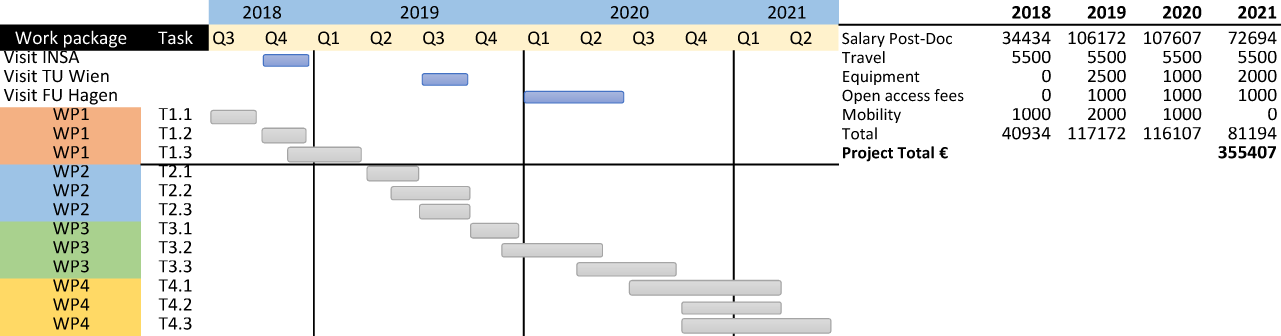
\includegraphics[scale=0.45]{fig/schedule.png}
	\caption{Time schedule for the project}
	\label{fig:schedule}
\end{figure}

\subsection{Budget}
The budget of the project is defined in Table 1.

\begin{wraptable}{r}{8cm}
\vspace{-3.2cm}
\small
\begin{tabular}{ | l | c | c |c |c |}
\hline
& {\textbf{2017}} & {\textbf{2018}} & {\textbf{2019}} & {\textbf{2020}} \\ \hline
{Salary Post-doc} 	& 34434 & 106172 & 107607 & 72694 \\ \hline
{Travel} 			& 5500 	& 5500 	& 5500 	& 5500  \\ \hline
{Equipment} 		& 0 	& 2500 	& 1000 	& 2000  \\ \hline
{Open access fees} 	& 0 	& 1000 	& 1000 	& 1000  \\ \hline
{Mobility} 			& 1000 	& 2000 	& 1000 	& 0  \\ \hline
{\textbf{Total}} 	& 40934 & 117172	& 116107 	& 81194  \\ \hline
{\textbf{Project total}} 	&  & 	&  	& 355407  \\ \hline
\end{tabular}
\caption*{Table 1: The budget of the project in euros}
\label{tab:budget}
\vspace{-0.5cm}
\end{wraptable}


\section{Research team and collaboration}
The team is internationally well connected and has established cooperation with several teams abroad and nationally. 
Our lab and the PI has worked within several international and national research projects such as RECOMP, ParallaX and INTERSYS with close ties to Finnish industry like Nokia, ABB, Kone, Ericsson etc.

\subsection{Collaboration}
The cooperation between Prof. Jean-Francois Nezan, INSA, Rennes, and \AA{}bo Akademi University has concentrated on the run-time management of dataflow networks, 
and has been executed through exchange of PhD students.
The PI visited INSA de Rennes for 4 months in 2013-2014, which resulted in two journal publications and two proceedings publications.\smallskip
INSA de Rennes has a strong background in tool support. 
The previously developed PREESM\footnote{http://preesm.sourceforge.net/website/} tool which was used to determine parallelism in data-flow programs to be used in a power optimizer developed by the PI in \AA{}bo Akademi University, and this work resulted in the best paper award at the 2014 DASIP conference.
A 3 month research mobility is planned early in the project to bring early tool integration of meta-data injection in WP1, and to determine the meta-data model needed for such tool integration.
In the later stages of the project, the utilization of PREESM is expected in form of a demonstration environment for WP4.\smallskip

A cooperation between Holmbacka and Prof. J\"{o}rg Keller at the FernUniversit\"{a}t in Hagen started in 2014, since when we have worked on energy efficient scheduling for multi-core systems. 
The lab group in Hagen has previously worked on performance models for very parallel systems such as the Intel SCC.
The PI is currently working in Hagen as a Post-doc exchange, and the cooperation with FernUni is currently very active.
One scientific journal and one proceedings publication about energy efficient scheduling has been published during this cooperation,
and this connection is therefore important mainly for the energy optimization in WP3 and the construction of the controller in WP3.
A 6 month visit is planned in the middle of WP3 during which the most critical part of the smart controller is to be constructed.
\smallskip

The PI has been cooperating with the Electronic Commerce Group in TU Wien led by Prof. Ivona Brandi\'{c} since spring 2015 inside the COST action IC1305 framework. 
Work on cost and energy efficient cloud scheduling was done by extending the Philharmonic cloud simulator\footnote{http://philharmonic.github.io/} created at TU Wien with a multi-core model developed by the PI at \AA{}bo Akademi University. 
A journal has been accepted in the IEEE Transactions journal as a result of this cooperation.
A 3 month research mobility is planned in the early WP2 firstly to evaluate complementary work and its suitability in our project.
Secondly, their expertise is of highest value early in WP2 after the meta-data framework has been established in WP1 in order to adapt and evaluate our framework in cloud environments.
\smallskip 

The most recent in the collaboration network is Dr. Alexandra Jimborean from Uppsala University in Sweden.
Their lab group is working on compile-time and runtime code analysis and transformation for performance and energy efficiency using LLVM.
Her group has developed a monitoring and feedback system for re-organizing instruction calls based on their memory intensity.
With this knowledge, their input is essential in WP2 when constructing the monitor system.
Also, our collaboration with overlapping expertise is needed in WP4 constructing the demonstrator.
No mobility is planned together with this team, but since Uppsala is located very close to Turku ad-hoc visits can be arranged without extensive pre-planning.


\subsection{Relation to strategic centers of research}
Since the Strategic Centres for Science, Technology and Innovation are being shut down, there is no concrete cooperation planned. 
However many of the SHOKs are planning new ways to continue their activities and since Prof. Lilius of the Embedded Systems Lab in \AA{}bo Akademi is a member of the FIMECC SG, 
he will have the opportunity to connect up the work in this project with the work done within FIMECC.


\section{Researcher training and research careers}
\textbf{Researcher training and supervision}: The supervision of PhD students are carried out as teamwork within participating senior researchers, 
but every student has also official supervisors with whom the student makes a study and research plans according to the university regulations. 
Each laboratory consists of researchers at various levels of their research career. 
It is paramount for all of them (including professors, researchers and staff) to periodically participate in the researcher training programs and renew their education/training.\smallskip

\textbf{Promotion of Research Career}: With the current application, we seek funding for a post-doc researcher to work full-time within the project. 
Combined with the international co-operation, exchange period and close interaction between participating institutes, the project gives to the involved post-doc good basis to proceed in the academic career after the project.

\section{Mobility plan}
The mobilities are planned as follows and illustrated in Figure \ref{fig:schedule}, but the exact details will be defined later in the project based on the availability of the collaborators and their time schedule.
\begin{itemize}
 \item Simon Holmbacka (PI) will visit Prof. Jean-Francois Nezan for 3 months in the beginning of WP1. \vspace{-0.3cm}
 \item Simon Holmbacka (PI) will visit Prof. Ivona Brandi\'{c} for 3 months in the beginning of WP2 \vspace{-0.3cm}
 \item Simon Holmbacka (PI) will visit Prof. J\"{o}rg Keller for 6 months in the middle of WP3. \vspace{-0.3cm}
\end{itemize}

\bibliographystyle{alpha}
{\footnotesize
\bibliography{sample}}

%----------------------------------------------------------------------------------------


\end{document}